\documentclass[parskip=full]{scrartcl}
\usepackage[utf8]{inputenc} % use utf8 file encoding for TeX sources
\usepackage[T1]{fontenc}    % avoid garbled Unicode text in pdf
\usepackage[german]{babel}  % german hyphenation, quotes, etc
\usepackage{hyperref}       % detailed hyperlink/pdf configuration
\hypersetup{                % ‘texdoc hyperref‘ for options
	pdftitle={Entwurf},%
	bookmarks=true,%
}
\usepackage{graphicx}       % provides commands for including figures
\usepackage{csquotes}       % provides \enquote{} macro for "quotes"
\usepackage{scrpage2}
\pagestyle{scrheadings}
\usepackage{float}

%\clearscrheadfoot
\ohead{BPTI: Gruppe 03=\{Niklas Metz, Felix Bachmann\}, Aufgabenblatt 2, WS 2017/18}

\begin{document}
	\setcounter{section}{0}
	\section{VGA-Ausgang}
		\subsection{Probleme bei der Implementierung}
			Das größte Problem bei dieser Aufgabe war die Darstellung der weißen Ränder auf dem Bildschirm. Nachdem wir mehrfach unser Programm überprüft haben und uns sicher waren, dass zumindest 3 von 4 Rändern dargestellt werden müssten, kamen wir auf die Idee, dass der Monitor das Problem darstellt. Als wir den Bildschirm richtig einstellten wurden die drei erwarteten Ränder gezeichnet. Um den letzten verbleibenden Rand zu zeichnen behoben wir noch ein Problem beim Zählen der Größe der Ausgabe.
			
		\subsection{Entwurf}
			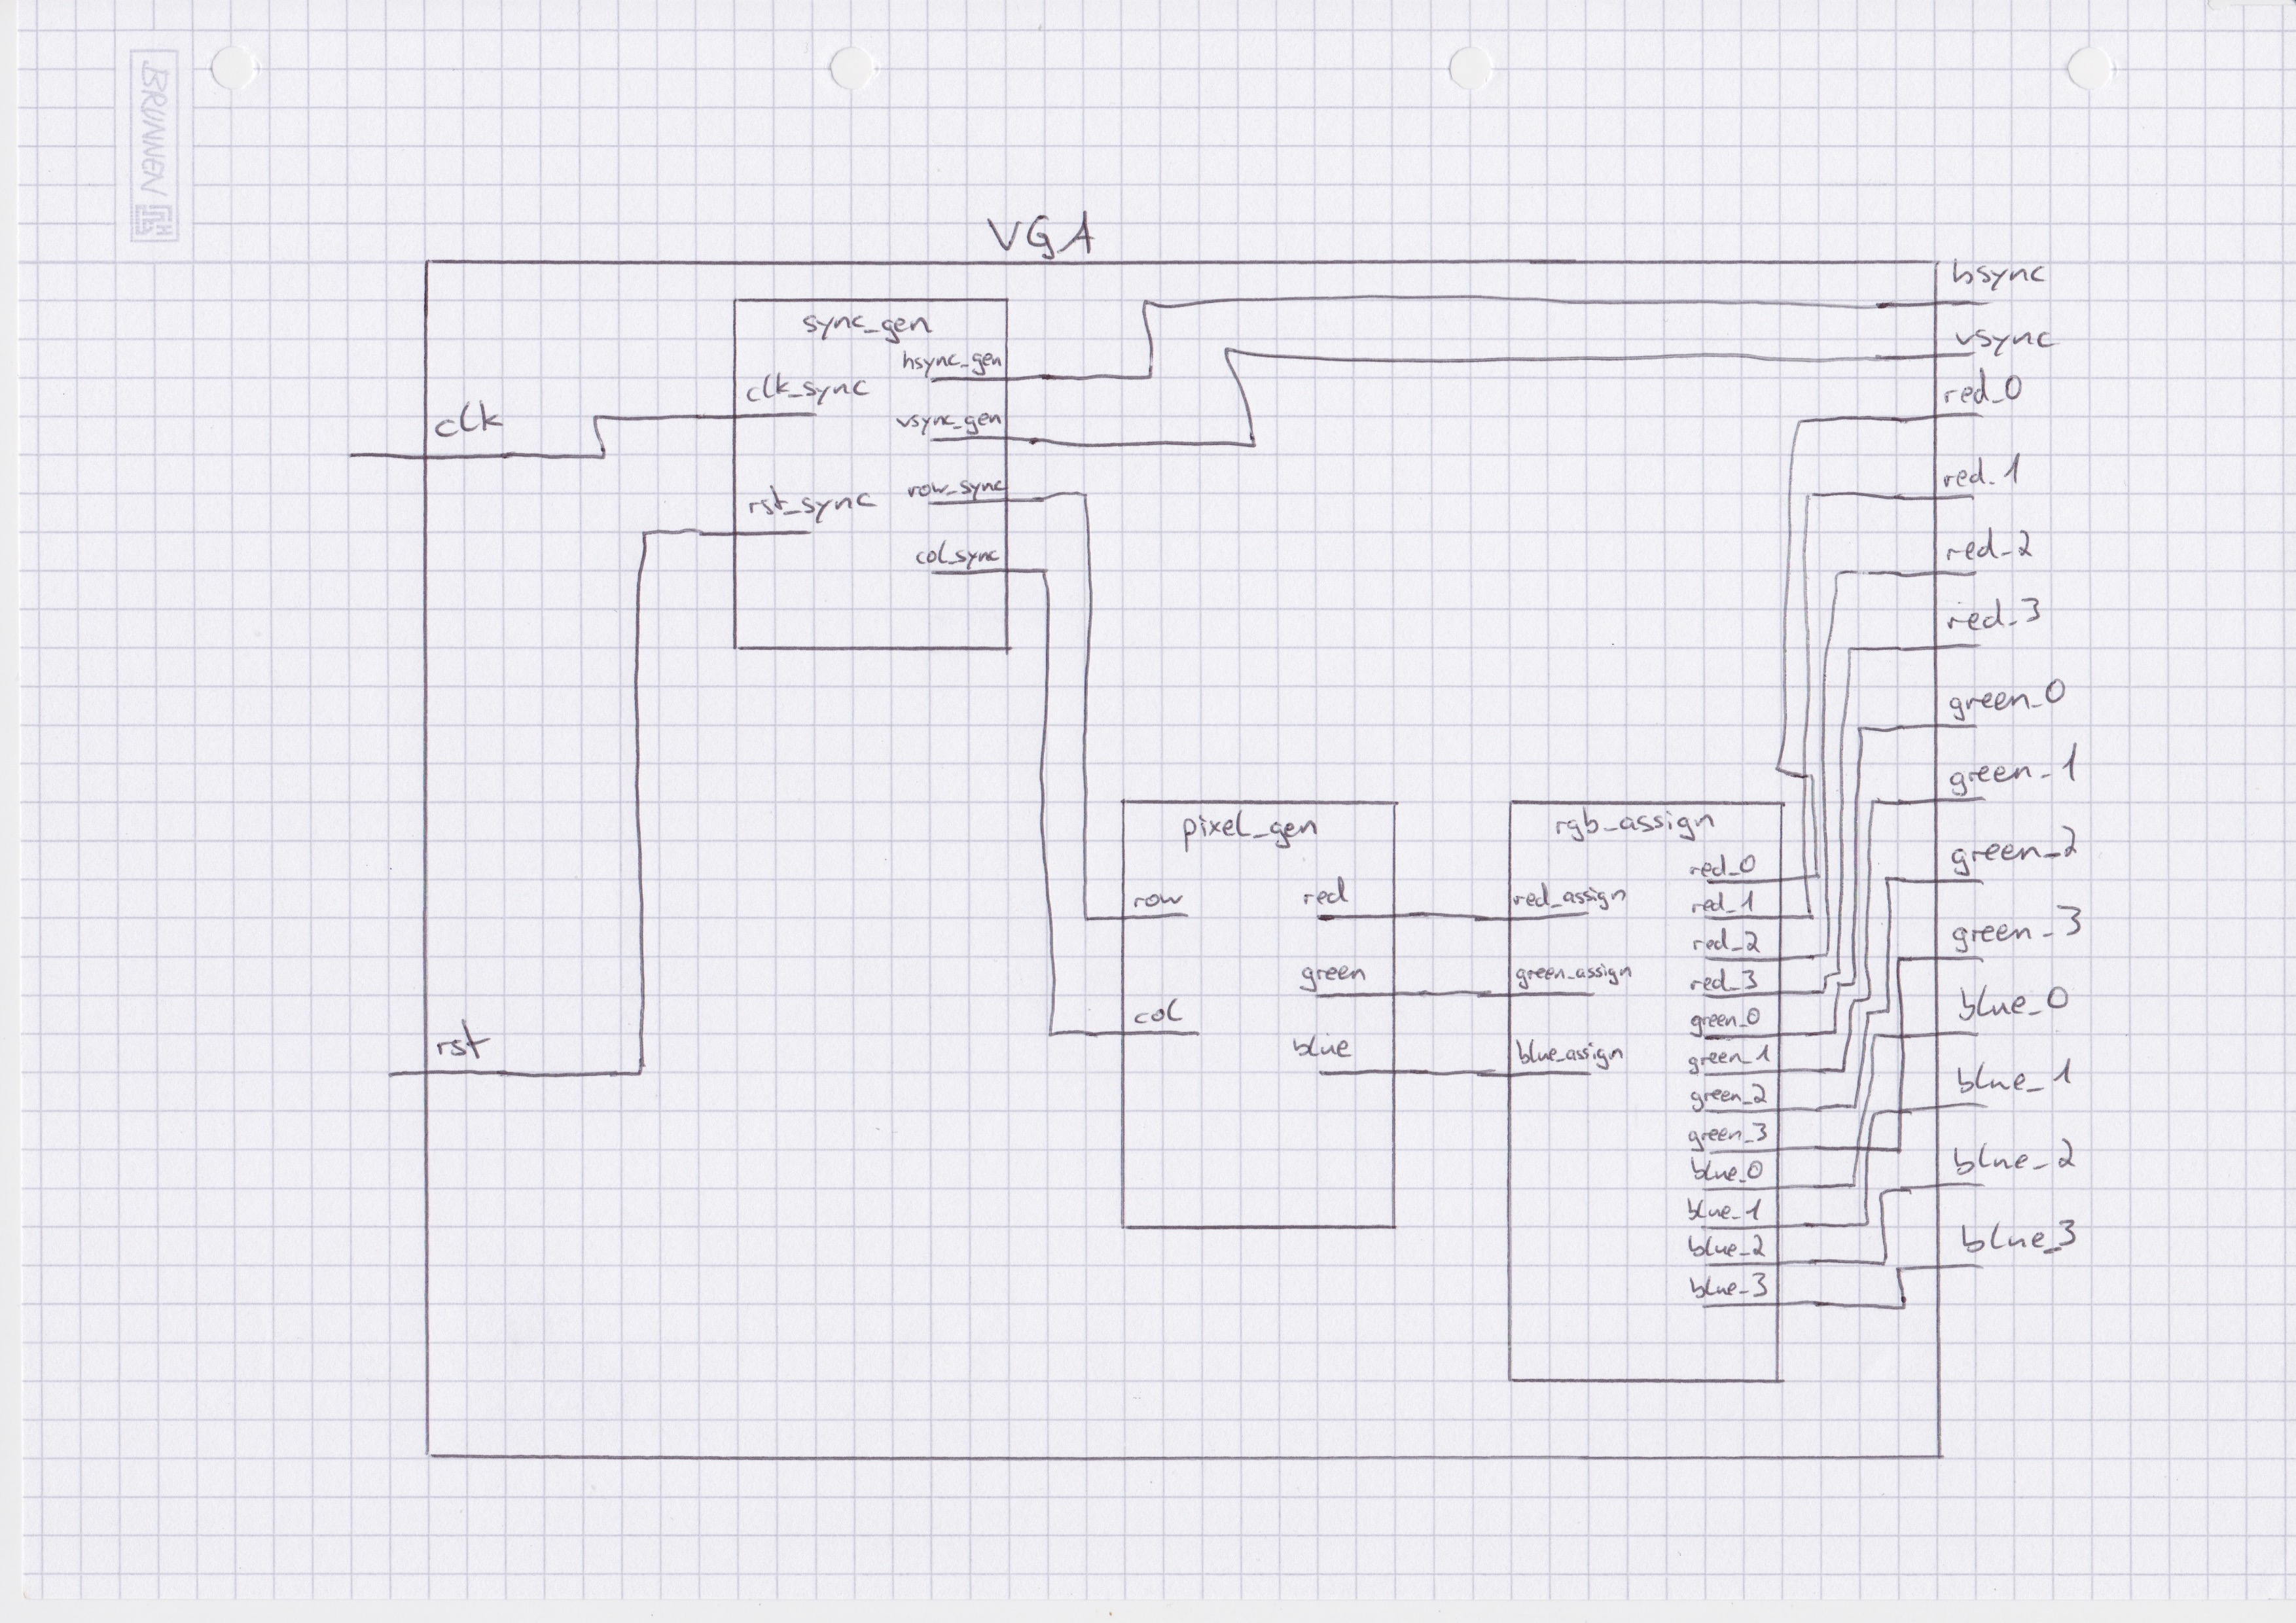
\includegraphics[scale=0.1]{Bilder/VGA.jpeg} \newline
			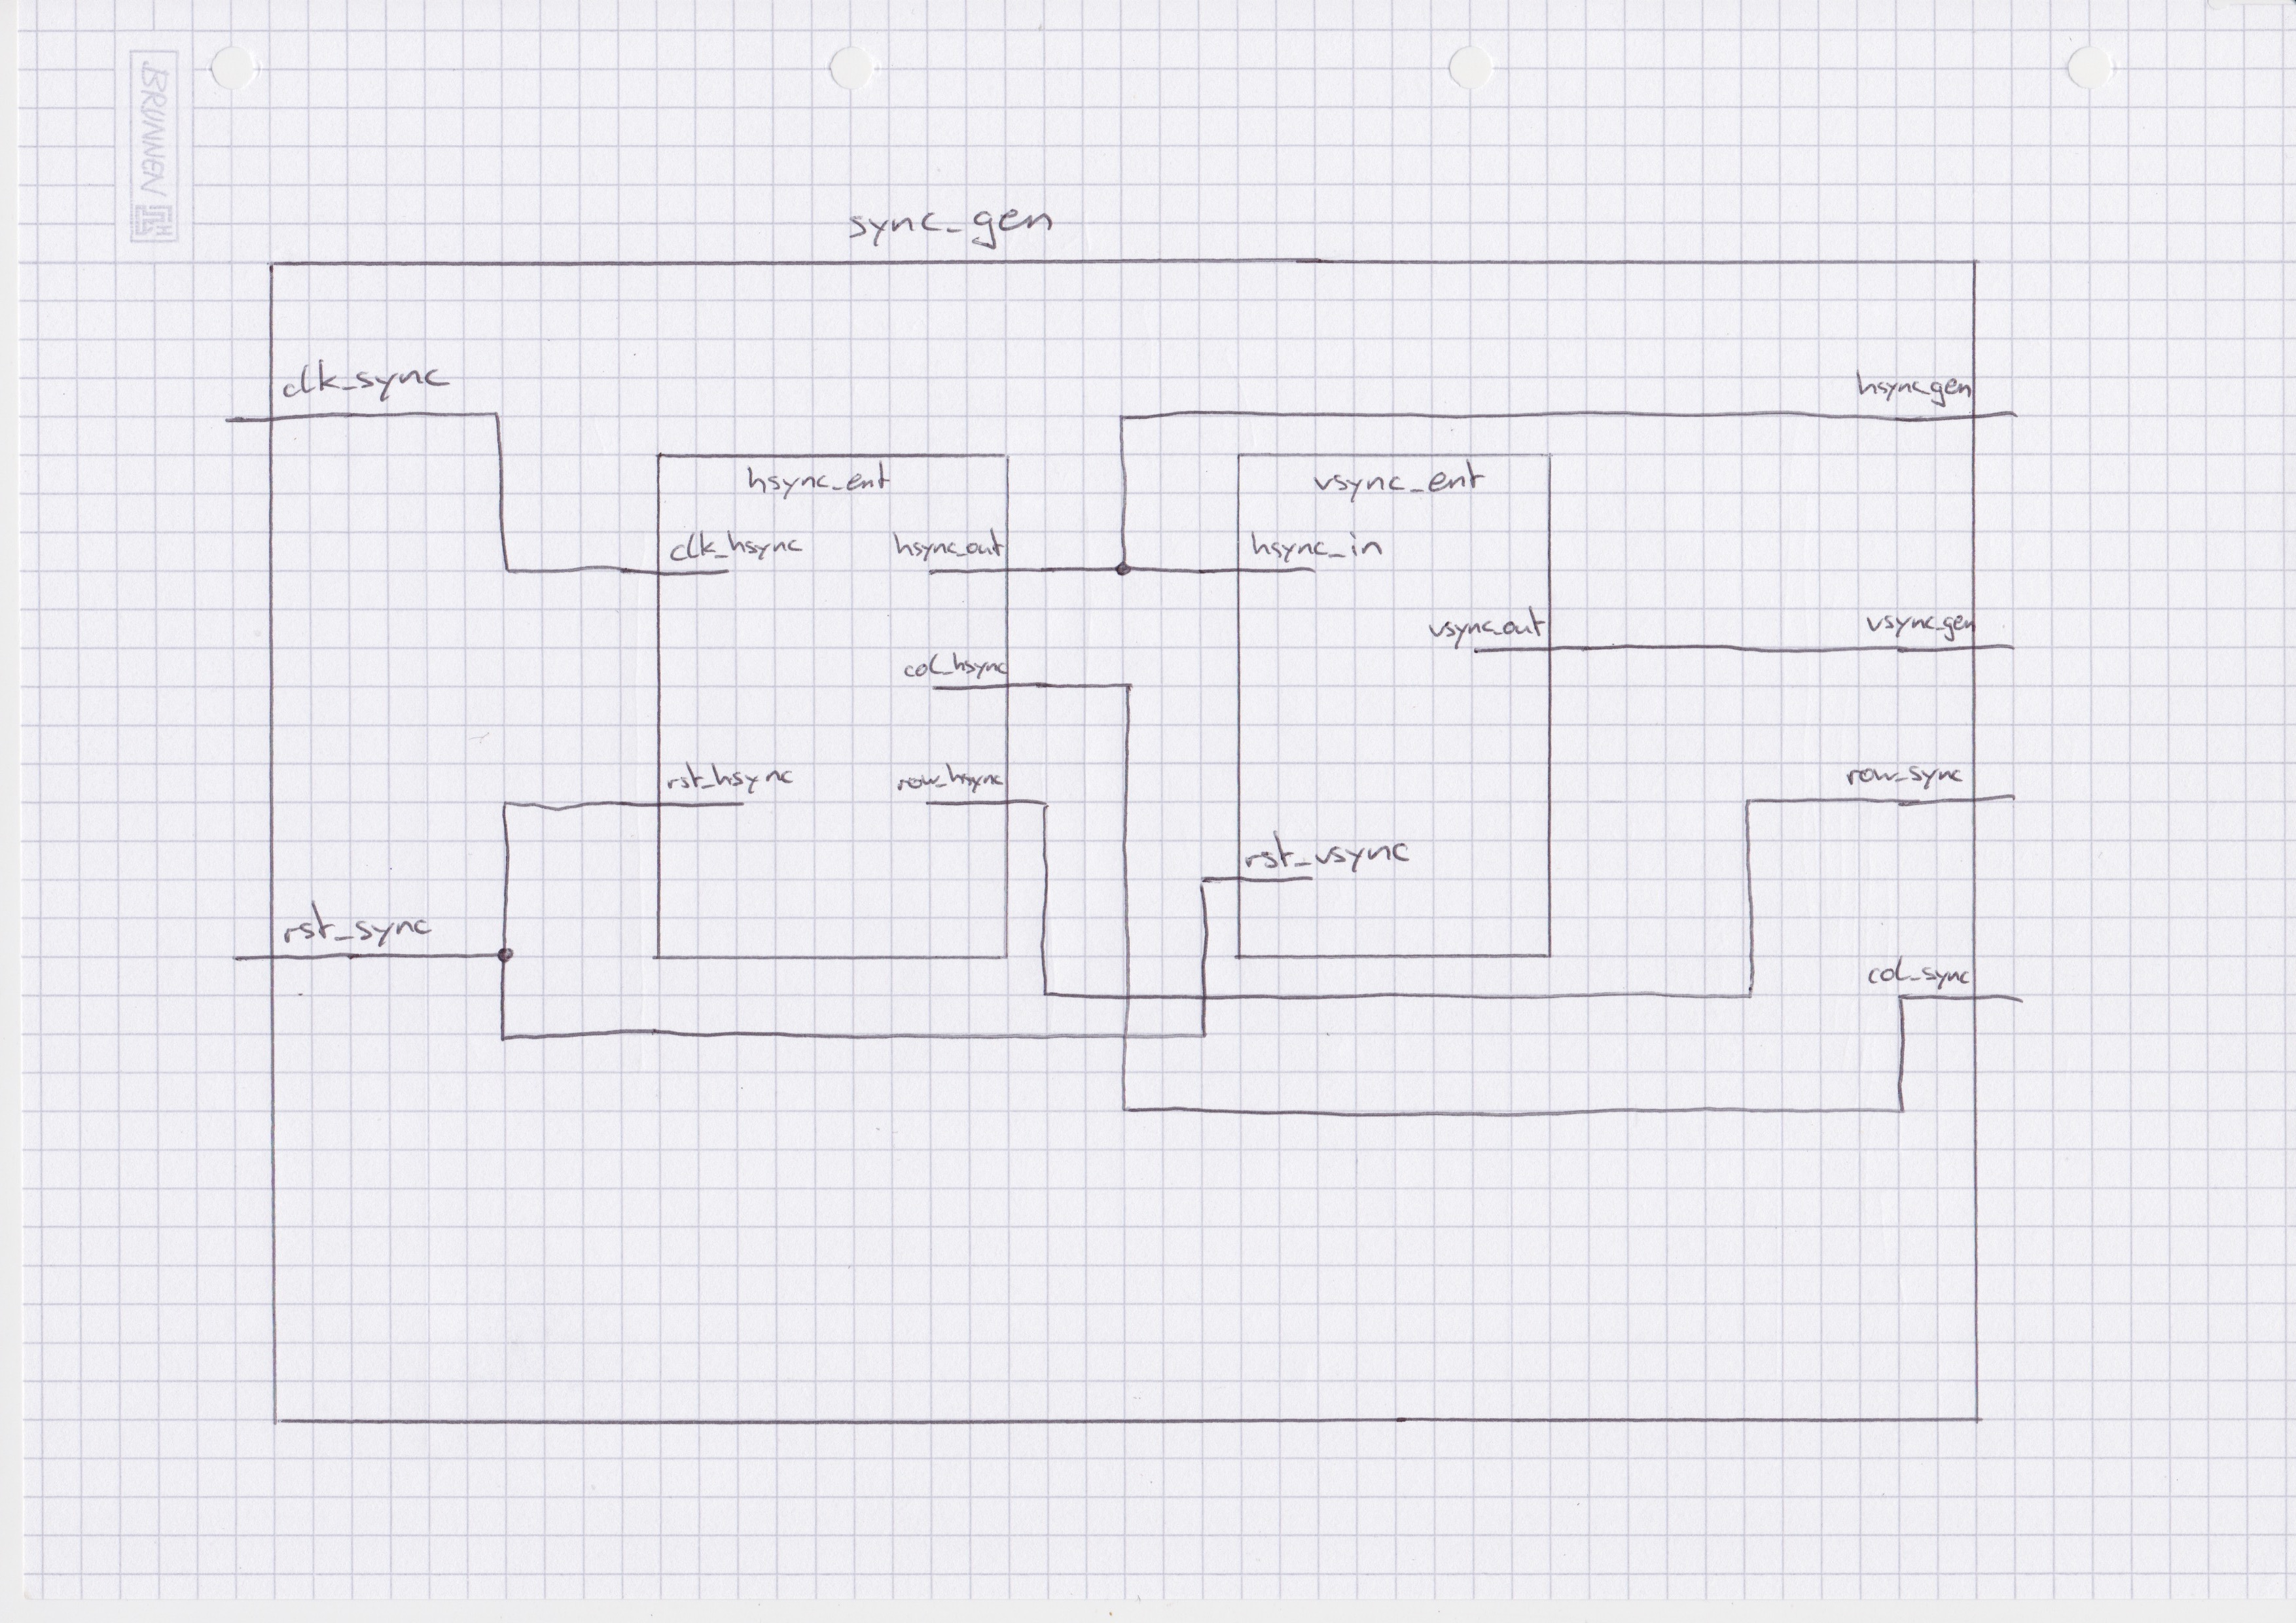
\includegraphics[scale=0.1]{Bilder/Sync_gen.jpeg}
			
		\subsection{Screenshots}
			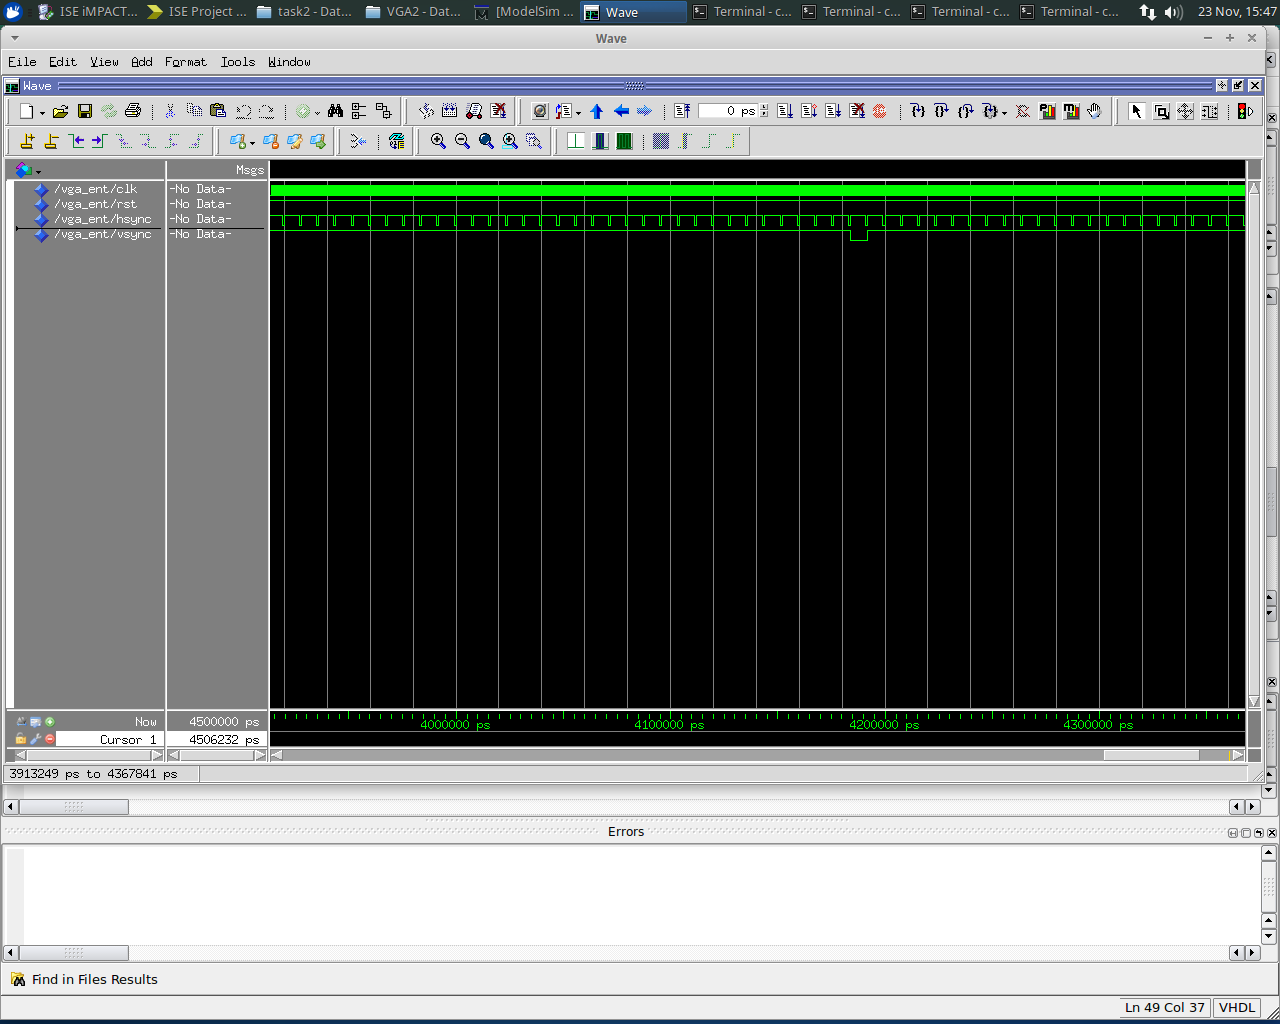
\includegraphics[scale=0.27]{Bilder/sync.png} \newline
			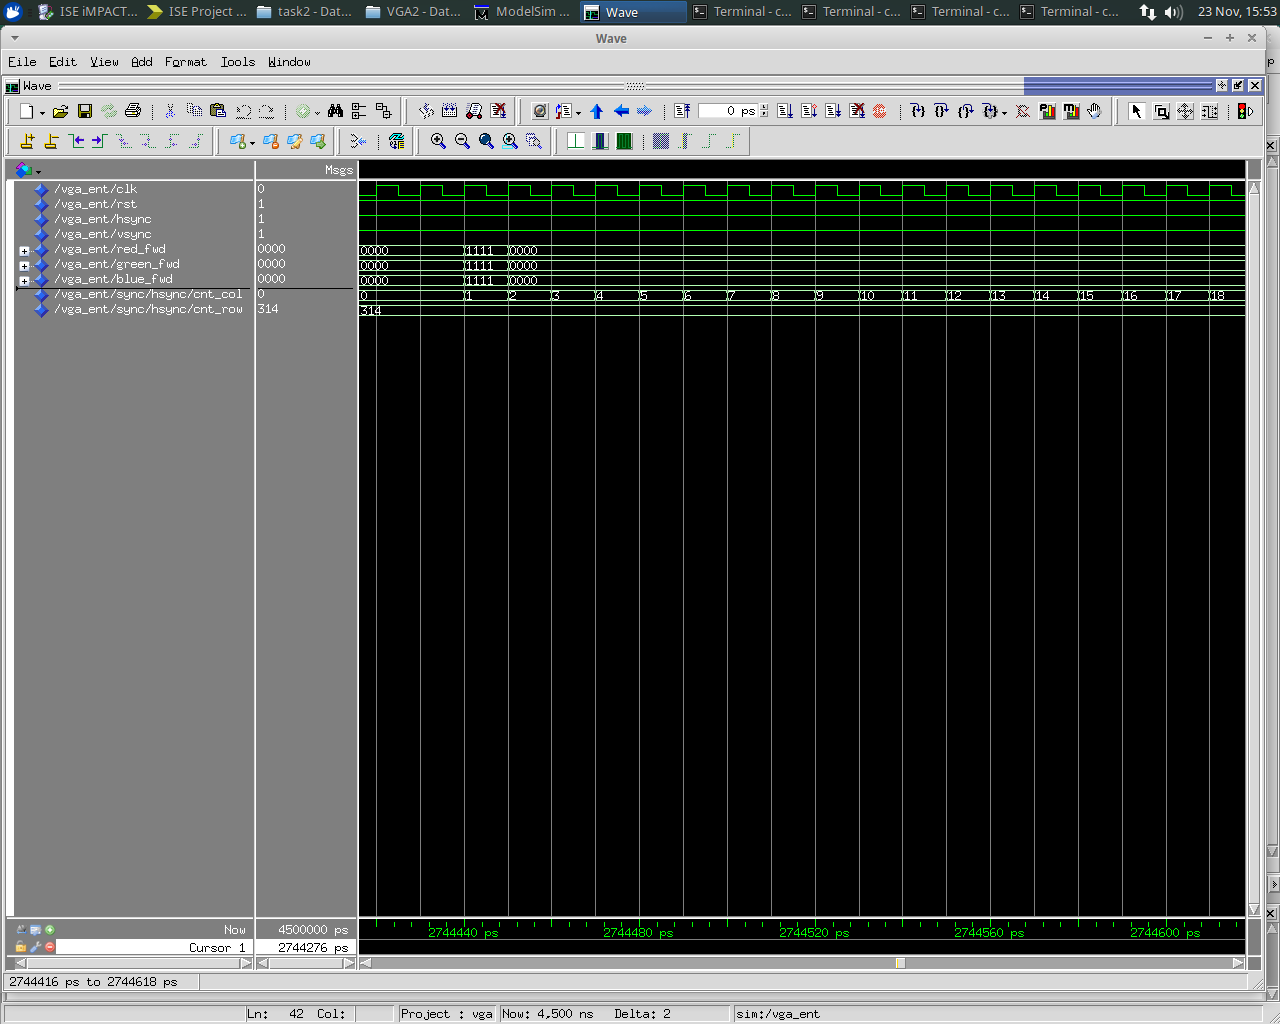
\includegraphics[scale=0.27]{Bilder/edge_white_rest_black.png}

	\section{Farbverlauf}
		
	\section{Rechteck}
		Die Ausgabe des Rechtecks stellte uns vor keine große Herausforderung. Ein Problem war, dass wir mehrfache Zuweisungen der Ausgänge hatten und somit kein rechter Rand des Rechtecks zu sehen war, sondern das Rechteck endlos nach rechts verlief.
	
	\section{Beeinflussung der Körper}
		Das Verschieben des Körpers mittels einer Eingabe war ebenfalls kein großes Problem. Einzig die Grenzfälle an den Seiten des Bildes bedurften mehr Gedanken. Bei den ersten Versuchen könnte man den Körper nicht bis ganz in die Ecken bewegen oder darüber hinaus. Dieses Problem war allerdings auch schnell behoben.
	
\end{document}
